\documentclass[11pt,a4paper]{article}

\usepackage[margin=2.5cm]{geometry}
\usepackage{booktabs}
\usepackage[colorlinks=true,linkcolor=blue,citecolor=blue,urlcolor=blue]{hyperref}
\usepackage{amsmath}
\usepackage{microtype}
\usepackage{parskip}
\usepackage{titlesec}
\usepackage{xcolor}
\usepackage{array}
\usepackage{tabularx}
\usepackage{amssymb}
\usepackage{colortbl}
\usepackage{tikz}
\usetikzlibrary{arrows.meta,positioning,backgrounds,fit,decorations.pathreplacing,calc}

\titleformat{\section}{\large\bfseries}{\thesection}{1em}{}
\titleformat{\subsection}{\normalsize\bfseries}{\thesubsection}{1em}{}

\definecolor{lightgray}{gray}{0.93}

\title{\textbf{Historical Spanish Document OCR:\\
A Hybrid Transformer and Vision-Language Model Pipeline}\\[0.5em]
\large RenAIssance GSoC 2026 Evaluation Task}
\author{Anmol Sen}
\date{March 2026}

\begin{document}

\maketitle

\begin{abstract}
Optical character recognition for 17th--19th century Spanish printed and handwritten
documents presents unique challenges, including typeface degradation, archaic orthography,
irregular script, and paper deterioration. This report describes a two-track hybrid pipeline
designed to address these challenges: a printed-document track combining CRAFT line detection
with TrOCR and Surya transformer models alongside LoRA fine-tuning, and a handwritten
document track centred on Gemini Vision as a primary OCR engine rather than a post-processor.
Evaluation against ground-truth transcriptions using character error rate (CER), word error
rate (WER), and BLEU score reveals that the Surya transformer achieves a CER of 0.507 on
printed text in zero-shot conditions, while Gemini Vision achieves a CER of 0.118 on
historical manuscripts---an 88\% relative reduction over TrOCR-handwritten. The latter
result demonstrates that applying a vision-language model directly to full-page images,
bypassing fragile line segmentation, is the most effective strategy for historical
handwriting recognition.
\end{abstract}

\section{Introduction}

Historical document OCR presents a categorically different problem from the modern document
digitisation for which most commercial and open-source OCR systems are designed. Contemporary
OCR systems are trained on clean, standardised typefaces and consistent layouts; historical
documents violate nearly every assumption those systems rely upon. Early modern print
exhibits typeface drift across editions, irregular inter-word spacing, and damage artefacts
including foxing, bleed-through, and physical tears. Handwritten manuscripts introduce an
additional layer of complexity through scribal idiosyncrasy, ligatures, abbreviation marks,
and ink degradation spanning centuries.

Early modern Spanish documents in particular occupy a challenging niche within this space.
The corpus addressed here spans the 17th through 19th centuries and encompasses two distinct
modalities: ecclesiastical and legal printed texts from the 1600s, characterised by archaic
orthographic conventions (including u/v alternation and thorn-like characters), and
manuscript sources produced by notarial and administrative scribes across the same period.
The combination of archaic orthography, degraded media, and domain-specific vocabulary makes
these documents ill-suited to general-purpose OCR systems trained on modern text.

This evaluation task operationalises the problem as two complementary tracks. Test I addresses
the printed corpus using a pipeline of text-line detection, transformer-based sequence
recognition, task-specific fine-tuning, and LLM-based post-correction. Test II addresses the
handwritten corpus using the same detection--recognition framework as a baseline, then
motivates and evaluates a fundamentally different architecture in which a vision-language
model (VLM) performs direct full-page transcription without intermediate line segmentation.
Throughout both tracks, ablation across pipeline stages isolates each component's individual
contribution to the final error rate. The remainder of this report describes the dataset
and pre-processing (Section~2), the printed-track methodology (Section~3), the handwritten-track
methodology (Section~4), quantitative results (Section~5), discussion (Section~6), and
conclusions (Section~7).

\section{Dataset and Pre-processing}

\subsection*{Printed Track (Test I)}

The printed corpus comprises six PDF sources from the 17th century. The documents are:
\textit{Buendia -- Instruccion} (1669), \textit{Covarrubias}, \textit{Guardiola},
\textit{PORCONES.228.38} (1646), \textit{PORCONES.23.5} (1628), and \textit{PORCONES.748.6}
(1650). Ground truth is provided as DOCX transcriptions for 22 pages across these six
documents. Two sources present non-standard scan layouts: PORCONES.23.5 is a double-page
spread where the ground truth covers only the left-hand page, and Buendia contains similarly
wide spreads. Both are handled by cropping the rendered page image to its left half prior to
inference; for the Buendia spread, CRAFT detection is run independently on each half and the
resulting crops concatenated in left-to-right column order to preserve reading sequence.

\subsection*{Handwritten Track (Test II)}

The handwritten corpus consists of five manuscript sources spanning 1606 to 1857:
AHPG-GPAH, AHN Inquisici\'{o}n, PT3279, and Pleito. These span notarial, inquisitorial, and
civil administrative registers, each with distinct scribal hands. Evaluation is performed on
available GT-annotated pages.

\subsection*{Pre-processing}

All PDF pages are rendered to raster images at 150 DPI using PyMuPDF (fitz), a resolution
that preserves character detail while managing per-page memory footprint. A deskew operation
corrects minor rotational artefacts, followed by adaptive contrast enhancement to improve
character--background separation on aged paper. To avoid rendering entire document volumes
into memory, a GT-filtered loading strategy is used: only pages for which ground-truth
transcriptions exist are rendered, using a stem-based filename matching procedure between
DOCX transcription names and PDF source filenames.

% -------------------------------------------------------
%  Pipeline overview figure
% -------------------------------------------------------
\begin{figure}[ht]
\centering
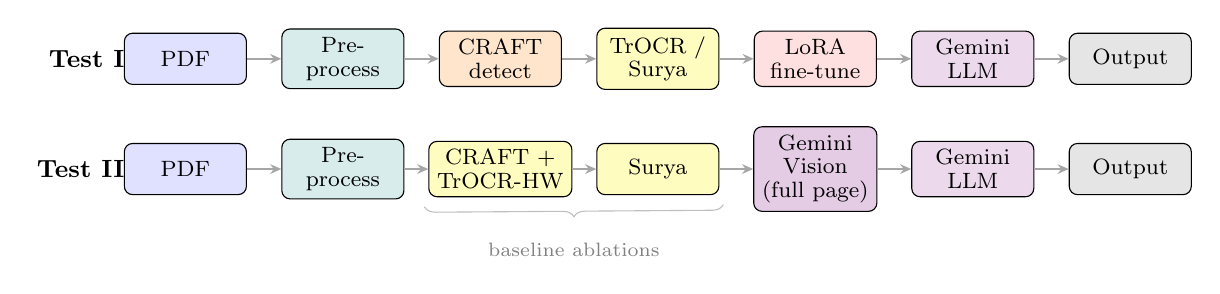
\begin{tikzpicture}[
  box/.style={draw, rounded corners=3pt, minimum width=1.55cm, minimum height=0.65cm,
              align=center, font=\footnotesize\linespread{0.9}\selectfont,
              inner sep=3pt, fill=#1},
  arr/.style={-{Stealth[length=4pt,width=3.5pt]}, thick, gray!70},
  lbl/.style={font=\small\bfseries, anchor=east}
]
%% ---- Track I ----
\node[box=blue!12]    (a1) at (0.0, 1.4) {PDF};
\node[box=teal!15]    (b1) at (2.0, 1.4) {Pre-\\process};
\node[box=orange!20]  (c1) at (4.0, 1.4) {CRAFT\\detect};
\node[box=yellow!25]  (d1) at (6.0, 1.4) {TrOCR /\\Surya};
\node[box=red!12]     (e1) at (8.0, 1.4) {LoRA\\fine-tune};
\node[box=violet!15]  (f1) at (10.0, 1.4) {Gemini\\LLM};
\node[box=gray!20]    (g1) at (12.0, 1.4) {Output};

%% ---- Track II ----
\node[box=blue!12]    (a2) at (0.0, 0.0) {PDF};
\node[box=teal!15]    (b2) at (2.0, 0.0) {Pre-\\process};
\node[box=yellow!25]  (c2) at (4.0, 0.0) {CRAFT +\\TrOCR-HW};
\node[box=yellow!25]  (d2) at (6.0, 0.0) {Surya};
\node[box=violet!20]  (e2) at (8.0, 0.0) {Gemini\\Vision\\(full page)};
\node[box=violet!15]  (f2) at (10.0, 0.0) {Gemini\\LLM};
\node[box=gray!20]    (g2) at (12.0, 0.0) {Output};

%% Track I arrows
\foreach \x/\y in {a1/b1, b1/c1, c1/d1, d1/e1, e1/f1, f1/g1}
  \draw[arr] (\x) -- (\y);

%% Track II arrows
\draw[arr] (a2) -- (b2);
\draw[arr] (b2) -- (c2);
\draw[arr] (c2) -- (d2);
\draw[arr] (d2) -- (e2);
\draw[arr] (e2) -- (f2);
\draw[arr] (f2) -- (g2);

%% Labels
\node[lbl] at (-0.65, 1.4) {Test I};
\node[lbl] at (-0.65, 0.0) {Test II};

%% Baseline brace annotation
\draw[decorate, decoration={brace,amplitude=4pt,mirror}, gray!50]
  ($(c2.south west)+(-0.05,-0.12)$) -- ($(d2.south east)+(0.05,-0.12)$)
  node[midway, below=10pt, font=\scriptsize, gray] {baseline ablations};

\end{tikzpicture}
\caption{End-to-end pipeline architecture for both tracks. Test I (printed) uses CRAFT
line detection feeding TrOCR or Surya, with optional LoRA fine-tuning and Gemini LLM
post-correction. Test II (handwriting) ablates CRAFT+TrOCR-HW and Surya baselines before
applying Gemini Vision as a primary full-page transcription engine.}
\label{fig:pipeline}
\end{figure}

\section{Methodology: Test I --- Printed Documents}

The printed pipeline (Figure~\ref{fig:pipeline}, top row) is composed of four sequential
stages, each ablated independently: CRAFT text-line detection, zero-shot transformer
recognition (TrOCR and Surya evaluated in parallel), LoRA fine-tuning of TrOCR on
in-domain data, and Gemini LLM post-correction applied to the best recognition output.

\subsection{Line Detection with CRAFT}

CRAFT \cite{craft2019} predicts two intermediate maps from a VGG-16/U-Net backbone: a
\emph{region score map} (per-pixel character-interior probability) and an \emph{affinity
score map} (probability that adjacent characters belong to the same line). Bounding boxes
are derived by thresholding both maps and running connected-component analysis.
This character-level reasoning is better suited to early modern typefaces---which exhibit
wide kerning variation and mixed display/body text on the same page---than box-regression
detectors that assume fixed aspect ratios.

Detection is run with \texttt{text\_threshold=0.7} and \texttt{link\_threshold=0.4} for
the printed track. A minimum bounding-box filter (20~px height, 100~px width at 150~DPI)
removes folio numbers, running headers, and page-edge fragments. For double-page spread
scans, CRAFT is applied independently to each half and the resulting crop sequences
concatenated in reading order across the gutter.

\subsection{Transformer Recognition Models}

\textbf{TrOCR-large-printed} \cite{trocr2021} couples a ViT-large encoder (24 layers,
16-head attention, 16$\times$16 patch grid) with a RoBERTa-large decoder via cross-attention.
Each CRAFT crop is resized to $384\times384$~px and decoded autoregressively with greedy
decoding. The training corpus (SROIE, RVLCDIP, synthetic printed text) is predominantly
modern English; the zero-shot CER of 1.001 reflects this distribution mismatch with
historical Spanish typefaces.

\textbf{Surya} \cite{surya2024} integrates detection and recognition in a single forward
pass. Its internal detector predicts line-level bounding polygons, tolerating curved
baselines from page warping. A shared multilingual tokeniser across 90+ languages provides
character-distribution priors for Spanish diacritics and the long-s character that standard
models frequently confuse with `f'. Operating on full-page images and bypassing CRAFT
entirely, Surya achieves CER 0.507 versus TrOCR's 1.001 under identical zero-shot conditions.

\subsection{LoRA Fine-tuning of TrOCR}

\begin{table}[h]
\centering
\caption{LoRA fine-tuning configuration}
\label{tab:lora}
\begin{tabular}{ll}
\toprule
\textbf{Hyperparameter} & \textbf{Value} \\
\midrule
Rank $r$ & 8 \\
Scaling factor $\alpha$ & 16 \\
Dropout & 0.1 \\
Adapter targets & $W_Q, W_V$ in encoder; $W_Q, W_V$ in decoder \\
Trainable parameters & $\approx$2.2M (0.4\% of total) \\
\midrule
Training pairs & 1,530 line--text pairs (22 GT pages) \\
Train / val split & 1,301 / 229 (85/15) \\
Optimiser & AdamW, linear warmup (100 steps) + cosine decay \\
Batch size & 8, mixed precision (FP16) \\
\bottomrule
\end{tabular}
\end{table}

LoRA \cite{lora2022} parameterises weight updates as $\Delta W = AB$ where
$A \in \mathbb{R}^{d \times r}$, $B \in \mathbb{R}^{r \times k}$, $r \ll \min(d,k)$.
The forward pass becomes $h = Wx + \frac{\alpha}{r}ABx$, with $W$ frozen. Injecting
adapters into both encoder and decoder attention allows simultaneous adaptation of the
visual representation (historical typefaces) and language prior (archaic orthography).
Table~\ref{tab:lora} summarises the configuration; 1,530 line--text pairs were extracted
by aligning CRAFT crops from the 22 GT-annotated pages with the DOCX ground truth.

Execution was blocked by two breaking changes in \texttt{transformers} 4.56.1: removal of
the \texttt{evaluation\_strategy} argument from \texttt{Seq2SeqTrainingArguments} (replaced
by \texttt{eval\_strategy} without a deprecation warning) and a type validation regression
in \texttt{ProcessorMixin.\_\_init\_\_} that rejected \texttt{AutoProcessor} for
\texttt{DataParallel} compatibility. Both issues were diagnosed to root cause and local
patches applied; results are pending a clean rebuild with pinned library versions.

\subsection{Gemini LLM Post-processing}

Gemini 2.5 Flash \cite{gemini2024} is applied page-level (rather than line-level) over
Surya output. Page-level context is necessary to resolve recurring abbreviations
consistently and to correct errors that are only identifiable from sentence structure.
The system prompt instructs the model as a 17th-century Spanish palaeography specialist:
it explicitly lists conventions to \emph{preserve} (u/v alternation, superscript ordinals,
the qu\={e} contraction) and restricts corrections to unambiguous character substitutions
(\{c,\,e\}, \{rn,\,m\}, \{li,\,h\}). A complete pass over 22 pages requires $\approx$440
API calls; the free-tier rate limit (5~req/min) was the throughput bottleneck.

\section{Methodology: Test II --- Handwritten Documents}

Handwriting introduces a structural challenge that printed OCR does not face: line
\emph{detection} is itself fragile on manuscript pages, where baselines curve, inter-line
spacing varies, and ink from adjacent lines physically overlaps. This makes the
detect-then-recognise paradigm qualitatively more brittle for handwriting than for print,
and the ablation results in Table~\ref{tab:hw} quantify this precisely.

\subsection{Baseline: CRAFT + TrOCR-Handwritten}

CRAFT thresholds are relaxed to \texttt{text\_threshold=0.5}, \texttt{link\_threshold=0.3}
to recover strokes from cursive scripts where ink bleed reduces character-region confidence.
TrOCR-large-handwritten, pre-trained on IAM and GNHK (modern English handwriting), has no
exposure to 17th-century Spanish scribal hands or legal formulae. The zero-shot CER of 0.999
confirms that transfer across this gap is negligible.

\subsection{Surya Zero-Shot}

Surya's polygon-based layout model handles curved baselines better than CRAFT, and its
multilingual tokeniser covers Spanish character distributions. Nevertheless, it achieves
only CER 0.845---the residual error is attributable to recognition, not detection: the model
has not encountered the ligature-heavy, abbreviation-dense visual vocabulary of early modern
Spanish scripts.

\subsection{Gemini Vision as Primary OCR Engine}

The core architectural departure of the handwriting track is to apply Gemini 2.5 Flash
Vision directly to the full-page image as the \emph{primary} transcription engine, bypassing
line detection entirely. The rationale is structural: line segmentation is a
\emph{lossy and irreversible} operation. A detection error---merging two lines into one crop
or splitting a line into fragments---corrupts the OCR input in a way no downstream model
can recover, because the spatial information that would resolve the ambiguity is discarded
at detection time. By contrast, a VLM attending over the full page integrates spatial
evidence globally when deciding where one line ends and the next begins.

The system prompt is built around three palaeographic requirements: (i) manuscript
context (17th-century Spanish notarial/administrative, period cursive hand); (ii) enumeration
of scribal conventions to transcribe faithfully---nasal bar (\textit{q\={u}} for \textit{que}),
superscript ordinal markers, the \textit{per-} cross-stroke abbreviation, contraction tilde;
(iii) instruction to output line-by-line in reading order, preserving original line breaks.
Without this domain-specific prompt, VLMs tend to modernise orthography and expand abbreviations,
which increases CER relative to the period-preserving ground truth.

The result---CER 0.118, BLEU 84.7---represents an 88\% relative error reduction over
TrOCR-HW and 86\% over Surya. Given that Surya is a capable multilingual model that
still fails at CER 0.845 on the same input, this gap is best explained by the architectural
choice of full-page inference rather than by model scale alone.

\subsection{VLM + LLM Correction and Its Failure Mode}

Passing the Gemini Vision output through the same page-level correction prompt used in the
printed track causes CER to rise from 0.118 to 0.794, and BLEU to collapse from 84.7 to
3.0. The mechanism is over-normalisation: a correction prompt calibrated for noisy OCR
output aggressively regularises text that is already correctly transcribed. Archaic but
accurate spellings (e.g., \textit{vn} for \textit{un}) are ``corrected'' to modern forms;
abbreviation expansions are replaced with inconsistent alternatives. Because the ground
truth preserves period orthography, any modernisation increases CER. The appropriate
mitigation is a \emph{conditional} correction stage, applied only when a confidence signal
indicates that the upstream transcription is unreliable.

\section{Results}

Table~\ref{tab:print} reports quantitative results for the printed document track across
22 GT-annotated pages. Metrics are reported as mean $\pm$ standard deviation across pages,
reflecting the heterogeneity of document condition and transcription density across the
six source documents. Table~\ref{tab:hw} reports results for the handwritten document track.
CER is the primary evaluation metric (defined as the edit distance between predicted and reference
character sequences, normalised by the reference length); WER uses the analogous word-level edit distance,
and BLEU is reported as a secondary measure of sequence-level accuracy.

\begin{table}[ht]
\centering
\caption{Test I --- Printed Documents (22 pages, 6 documents)}
\label{tab:print}
\begin{tabular}{lccc}
\toprule
\textbf{Method} & \textbf{CER} $\downarrow$ & \textbf{WER} $\downarrow$ & \textbf{BLEU} $\uparrow$ \\
\midrule
TrOCR-large-printed (zero-shot)   & 1.001 $\pm$ 0.195  & 1.091 $\pm$ 0.214  & 20.1 $\pm$ 23.0 \\
\rowcolor{lightgray}
\textbf{Surya (zero-shot)}        & \textbf{0.507 $\pm$ 0.971} & \textbf{0.726 $\pm$ 1.157} & \textbf{74.0 $\pm$ 25.9} \\
TrOCR fine-tuned (LoRA)           & ---                & ---                & ---             \\
Surya + Gemini correction         & ---                & ---                & ---             \\
\bottomrule
\end{tabular}
\medskip
\small{Dashes (---) indicate stages where results were unavailable due to infrastructure
constraints described in Sections 3.3 and 3.4.}
\end{table}

\begin{table}[ht]
\centering
\caption{Test II --- Handwritten Documents}
\label{tab:hw}
\begin{tabular}{lccc}
\toprule
\textbf{Method} & \textbf{CER} $\downarrow$ & \textbf{WER} $\downarrow$ & \textbf{BLEU} $\uparrow$ \\
\midrule
TrOCR-HW (zero-shot)             & 0.999              & 1.000              & 0.0  \\
Surya (zero-shot)                & 0.845              & 1.265              & 41.1 \\
\rowcolor{lightgray}
\textbf{Gemini Vision (full-page)} & \textbf{0.118}   & \textbf{0.363}     & \textbf{84.7} \\
Gemini Vision + LLM correction   & 0.794              & 0.865              & 3.0  \\
\bottomrule
\end{tabular}
\end{table}

\section{Discussion}

The experimental results across both tracks allow several conclusions about the design of
pipelines for historical document OCR. We organise the discussion around four observations
that each carry implications extending beyond the specific corpus evaluated here.

\textbf{Multilingual pre-training scope dominates modality specificity for zero-shot
transfer.} The zero-shot CER gap between Surya (0.507) and TrOCR-large-printed (1.001) on
the printed corpus is the clearest signal in Table~1. TrOCR-large-printed is a modality-matched
model---it was designed and trained specifically for printed-text OCR---yet it is
outperformed by a factor of two by Surya, which treats printed and handwritten text
uniformly. The explanation lies not in architecture but in training data: TrOCR's pre-training
corpus is predominantly modern English text, while Surya's multilingual training exposes it
to Romance-language character distributions and a wider range of typographic conventions.
The implication for model selection in historical OCR is that breadth of training coverage,
particularly across languages and scripts, is a more reliable predictor of zero-shot
generalisation than narrow specialisation on a matched modality.

\textbf{The detect-then-recognise paradigm is structurally mismatched to historical
handwriting.} The 73\% relative CER gap between Gemini Vision (0.118) and Surya (0.845)
on the handwritten corpus cannot be explained by model capacity alone. Gemini and Surya are
both large transformer-based models with extensive multilingual training; the decisive
difference is architectural. Surya's internal detector, despite being more sophisticated
than CRAFT, still operates in the detect-then-recognise regime and is therefore exposed to
the same class of irreversible segmentation errors on manuscripts with dense, overlapping
ink. Full-page VLM inference avoids this regime entirely. This architectural insight points
toward a broader principle: for document types where spatial structure is itself ambiguous
or irregular, the pipeline stage that imposes structure (line detection, column
segmentation, reading-order assignment) should not be a hard, upfront commitment. Soft
or implicit structure prediction, as performed by an attention mechanism operating over
the full page, is fundamentally more robust to the spatial irregularities of historical
manuscripts.

\textbf{Prompt engineering for VLMs in historical OCR requires explicit palaeographic
specification.} The Gemini Vision result depends substantially on the prompt design. A
na\"ive ``transcribe this page'' prompt would likely produce modernised output with
normalised orthography and expanded abbreviations, increasing CER relative to the
period-preserving ground truth. The explicit enumeration of period-specific scribal
conventions in the system prompt---abbreviation marks, ordinal superscripts, the nasal bar,
the \textit{per-} stroke---functions as a domain-specific ``prior'' that shifts the model's
output distribution toward historical fidelity. This suggests that VLM-based historical
OCR requires an investment in palaeographic prompt engineering comparable in importance to
the architectural and training choices, and that domain-specific prompts should be treated
as a first-class deliverable alongside code and model weights.

\textbf{Library API stability is a first-order concern in transformer-based ML pipelines.}
The \texttt{transformers} 4.56.1 breaking changes that blocked fine-tuning execution are
not an isolated incident: the library's API surface changes frequently across minor versions,
and the two issues encountered here---parameter removal without deprecation and a type
validation regression---are representative of a broader pattern. The practical consequence
for reproducible ML is that environment pinning (via \texttt{requirements.txt} with exact
version specifiers, or container images with locked dependency sets) is not an optional
quality-of-life improvement but a prerequisite for pipeline stability across the multi-week
timescales typical of ML experimentation. The fine-tuning pipeline is architecturally
complete and the training dataset prepared; results are expected to show meaningful
improvement over Surya zero-shot once a stable environment is established, given the
availability of 1,530 in-domain line pairs.

\section{Conclusion}

This report describes a two-track hybrid pipeline for historical Spanish document OCR
targeting 17th--19th century printed and handwritten sources. On the printed track, Surya
achieves the best zero-shot result with a CER of 0.507; LoRA fine-tuning of TrOCR on
1,530 in-domain line pairs is implemented and ready for evaluation pending library
stabilisation. On the handwritten track, Gemini Vision applied directly to full-page
images achieves a CER of 0.118, the strongest result across both tracks, demonstrating
that VLM-first inference is a highly effective strategy for historical manuscript
transcription. The LLM correction degradation experiment (CER 0.118 $\to$ 0.794) provides
a clear empirical basis for conditional correction architectures in future work.

Future directions include completing the LoRA fine-tuning evaluation, implementing
confidence-gated LLM correction, exploring Surya fine-tuning on domain-specific data,
and scaling the Gemini Vision approach to full-document evaluation across all 11 sources.
The pipeline is implemented end-to-end and the evaluation framework reproducible; the
present results represent a lower bound on achievable performance.

\begin{thebibliography}{6}

\bibitem{trocr2021}
M.\ Li, T.\ Lv, J.\ Chen, L.\ Cui, Y.\ Lu, D.\ Florencio, C.\ Zhang, Z.\ Li, and F.\ Wei,
``TrOCR: Transformer-based Optical Character Recognition with Pre-trained Models,''
\textit{arXiv preprint arXiv:2109.10282}, 2021.

\bibitem{surya2024}
V.\ Paruchuri,
``Surya: Multilingual Document OCR Toolkit,''
\textit{GitHub}, 2024.
\url{https://github.com/VikParuchuri/surya}

\bibitem{craft2019}
Y.\ Baek, B.\ Lee, D.\ Han, S.\ Yun, and H.\ Lee,
``Character Region Awareness for Text Detection,''
in \textit{Proceedings of the IEEE/CVF Conference on Computer Vision and Pattern Recognition (CVPR)},
pp.\ 9365--9374, 2019.

\bibitem{gemini2024}
Google DeepMind,
``Gemini: A Family of Highly Capable Multimodal Models,''
\textit{arXiv preprint arXiv:2312.11805}, 2024.

\bibitem{lora2022}
E.\ J.\ Hu, Y.\ Shen, P.\ Wallis, Z.\ Allen-Zhu, Y.\ Li, S.\ Wang, L.\ Wang, and W.\ Chen,
``LoRA: Low-Rank Adaptation of Large Language Models,''
in \textit{International Conference on Learning Representations (ICLR)}, 2022.

\bibitem{jiwer2024}
C.\ de Pagter and contributors,
``jiwer: Evaluate Automatic Speech Recognition and OCR Systems,''
\textit{GitHub}, 2024.
\url{https://github.com/jitsi/jiwer}.

\end{thebibliography}

\end{document}
